\section{Algorithms and problems}
Since the ancient age, there has always been the need of describing the sequence of activities needed to perform a specific task [...], to which we refer with the name of \textit{Algorithm}. The most ancient known example of this dates back to the Babylonians, who invented algorithms to perform the factorization and the approximation of the square root [...]. Regardless of the specific details of each algorithm, one needs to use some kind of language  to define the sequence of steps to perform. In the past people used natural language to describe such steps but, with the advent of the computer era, the choice of the language has been strictly connected with the possibility of its implementation [...]. Natural languages are not suitable for the implementation, as they are known to be verbose and ambiguous. For this purpose, several kind of formal solutions have been employed, which are described below.

\paragraph{Flow charts}
A flow chart is a diagram where the steps of an algorithm are defined by using boxes of different kinds, connected by arrows to define their ordering in the sequence. The boxes are rectangular-shaped if they define an \textit{activity} (or processing step), while they are diamond-shaped if they define a \textit{decision}. An example of a flow chart describing how to sum the numbers in a sequence is described in Figure \ref{fig:ch1_flow_chart}.

\begin{figure}
	\centering
	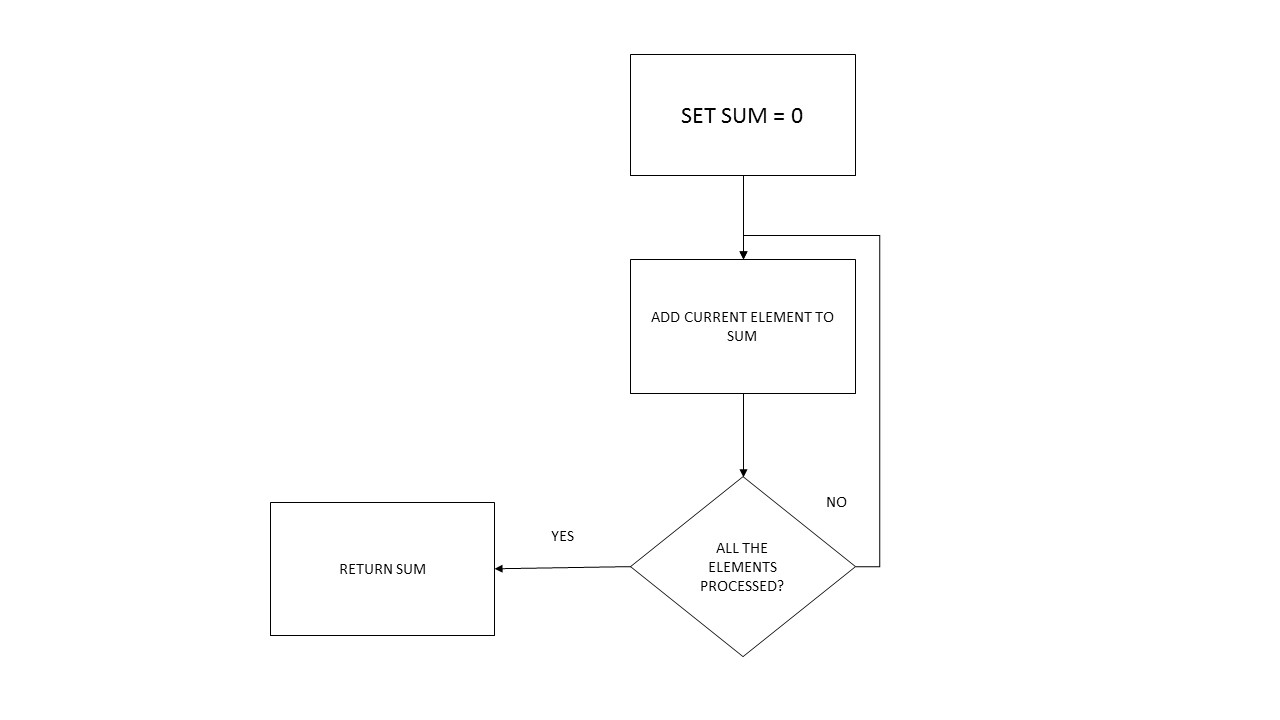
\includegraphics[width = \textwidth]{Figures/flow_chart}
	\caption{Flow chart for the sum of a sequence of numbers}
	\label{fig:ch1_flow_chart}
\end{figure}

\paragraph{Pseudocode}
Pseudocode is a semi-formal language that might contain also statements expressed in natural language and omits system specific code like opening file writers, printing messages on the standard output, or even some data structure declaration and initialization. It is intended mainly for human reading rather than machine reading. The pseudocode to sum a sequence of numbers is shown in Algorithm \ref{alg:ch1_pseudocode}.

\begin{algorithm}
	\caption{Pseudocode to perform the sum of a sequence of integer numbers}
	\label{alg:ch1_pseudocode}
	\begin{algorithmic}
		\Function{SumIntegers}{$l \text{ list of integers}$}
			\State $sum \gets 0$
			\ForAll {$x \text{ in } l$}
				\State $sum \gets sum + x$
			\EndFor
			\State \Return $sum$
		\EndFunction
	\end{algorithmic}
\end{algorithm}

%It might be necessary to make a section about how an algorithm is expressed as pseudo-code and then it has to be implemented in a programming language. An introduction section on how expressing algorithm in history has evolved might be a good idea.

\section{Programming languages}
A programming language is a formal language that is used to define instructions that a machine, usually a computer, must perform in order to produce a result through computation [...]. There is a variety of taxonomies used to classify programming languages [...], but all of them are considering four main characteristics [...]: the level of abstraction, or how close to the specific targeted hardware they are, and the domain, which defines the range of applicability of a programming language. In the following sections we give an exhaustive explanation of the aforementioned characteristics.

\subsection{Low-level programming languages}
A low-level programming language is a programming language that provides little to no abstraction from the hardware architecture of a processor [...]. This means that it is strongly connected with the instruction set of the targeted machine, the set of instructions a processor is able to execute. These languages are divided into two sub-categories: \textit{first-generation} and \textit{second-generation} languages [...]:

\subsubsection*{First-generation languages}
\textit{Machine code} falls into the category of first-generation languages. In this category we find all those languages that do not require code transformations to be executed by the processor. These languages were used mainly during the dawn of computer age and are rarely employed by programmers nowadays [...]. Machine code is made of stream of binary data, that represents the instruction codes an their arguments [...]. Usually this stream of data is treated by programmers in hexadecimal format, which is then remapped into binary code. The programs written in machine code were once loaded into the processor through a front panel, a controller that allowed the display and alteration of the registers and memory (see Figure \ref{fig:ch1_front_panel}). An example of machine code for a program that computes the sum of a sequence of integer numbers can be seen in Listing \ref{lst:ch1_machine_code}.

\begin{figure}
	\centering
	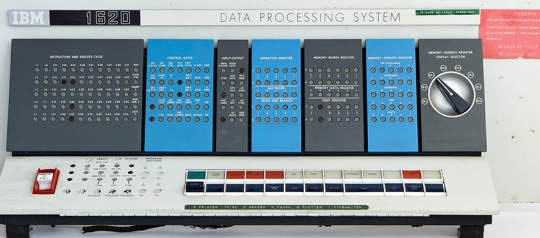
\includegraphics[width = \textwidth]{Figures/ch1_front_panel}
	\caption{Front panel of IBM 1620}
	\label{fig:ch1_front_panel}
\end{figure}


\begin{lstlisting}[caption = Machine code to compute the sum of a sequence of numbers, label = lst:ch1_machine_code]
Here put an example of hexadecimal machine code generated using C++ (for example sum of an array of integers)
\end{lstlisting}

\subsubsection*{Second-generation languages}
The languages in this category provides an abstraction layer over the machine code by expressing processor instructions with mnemonic names both for the instruction code and the arguments. For example the arithmetic sum instruction \texttt{add} is the mnemonic name for the instruction code \texttt{0x00} in \texttt{x86} processors. Among these languages we find \textit{Assembly}, that is mapped with an \textit{Assembler} to machine code. The Assembler can load directly the code or link different \textit{object files} to generate a single executable by using a \textit{linker}. An example of assembly \texttt{x86} code corresponding to the machine code in Listing \ref{lst:ch1_machine_code} can be found in Listing \ref{lst:ch1_assembly_code}.

\begin{lstlisting}[caption = Assembly x86 code to compute the sum of a sequence of numbers, label = lst:ch1_assembly_code]
Example of Assembly x86 code generated using c++
\end{lstlisting}

\subsubsection*{Advantages and disadvantages}
Writing a program in low-level programming languages have been known to produce programs that are generally more efficient than their high-level counterparts [...]. However, the high-performance comes at great costs: (\textit{i}) the programmer must be an expert of the underlying architecture and of the specific instruction set of the processor, (\textit{ii}) the program loses portability because the low-level code is tightly bound to the specific hardware architecture it targets, and (\textit{iii}) the logic and readability of the program is hidden among the details of the instruction set itself.

\subsection{High-level programming languages}
A high-level programming language is a programming language that offers a high level of abstraction from the specific hardware architecture of the machine [...]. Unlike machine code (and in some way also assembly), high-level languages are not directly executable by the processor and they require some kind of translation process into machine code. The level of abstraction offered by the language defines how high level the language is. Several categories of high-level programming language exist, but the main one are described below.

\subsubsection*{Imperative programming languages}
\textit{Imperative programming languages} model the computation as a sequence of statements that alter the state of the program (usually the memory state). A program in such languages consists then of a sequence of \textit{commands}. Notable examples are FORTRAN, C, and PASCAL. An example of the program used in Listing \ref{lst:ch1_machine_code} and \ref{lst:ch1_assembly_code} written in C can be seen in Listing \ref{lst:ch1_c_code}

\begin{lstlisting}[caption = C code to compute the sum of a sequence of numbers, label = lst:ch1_c_code]
Code for integer sequence sum in C
\end{lstlisting}

\subsection*{Declarative programming}

\textbf{Section layout}
\begin{itemize}[noitemsep]
	\item Classification of programming languages.
	\item Motivation for programming languages.
	\item Understanding of programming languages
\end{itemize}

\section{Compilers}
\begin{itemize}[noitemsep]
	\item Origin of compilers.
	\item Reason of compilers.
	\item Requirements of compilers.
\end{itemize}

Connect to the previous section by explaining why compilers were born and how you design and build a compiler.

\section{Meta-compilers}
\begin{itemize}[noitemsep]
	\item History of meta-compilers
	\item Motivation behind meta-compilers.
	\item Requirements of meta-compilers.
\end{itemize}
 Idea behind meta compilers. Introduction of the first META-languages family of meta-compilers, parser generators, then RML and other meta-compilers based on natural semantics. Main requirements of a meta-compiler.

\section{Scientific relevance}

Discuss about the few existing results in the field, and performance vs language customization issues (fixed rule representation, fixed symbol table structure, etc.).

\section{Problem statement}

Can we build a meta-compiler that is able to implement a language in less lines of codes than the hard-coded compiler, and at the same time have good performance?